\documentclass{article}

\usepackage{arxiv}
\usepackage[utf8]{inputenc} % allow utf-8 input
\usepackage[T1]{fontenc}    % use 8-bit T1 fonts
\usepackage{hyperref}       % hyperlinks
\usepackage{url}            % simple URL typesetting
\usepackage{booktabs}       % professional-quality tables
\usepackage{amsfonts}       % blackboard math symbols
\usepackage{amsmath}        % mathematical operators and formatting
\usepackage{nicefrac}       % compact symbols for 1/2, etc.
\usepackage{microtype}      % microtypography
\usepackage{graphicx}
\usepackage{float}

\raggedbottom

\title{Small Data Machine Learning: The Trilemma of Low-Sample Tabular Regimes}

\author{
  \textbf{Ilya Emelyanov}\footnotemark[1] \\
  \texttt{1820262250@bit.edu.cn}
  \and
  \textbf{Dmitrii Dobrydin} \\
  \texttt{1820262226@bit.edu.cn}
  \and
  \textbf{Muhammad Hamza} \\
  \texttt{7520250266@bit.edu.cn} \\[2ex]
  \textbf{Beijing Institute of Technology, Beijing, China}
}

\begin{document}
\maketitle
\footnotetext[1]{Corresponding author.}

\begin{abstract}
Machine learning on small tabular datasets ($n < 1000$) is governed by the \textit{Trilemma of Small Data Learning}: the inability to simultaneously achieve low variance, low bias, and calibrated uncertainty without depleting scarce training signals via validation splits. Rather than proposing a universal framework, this paper formalizes these mathematical bottlenecks and evaluates two lightweight, zero-tuning algorithmic baselines as case studies alongside existing targeted paradigms such as pre-trained in-context tabular foundation models (TabPFN / TabPFN v2). For robust classification, we analyze SmallGBM, which combines size-adaptive median leaf aggregation, MAD empirical Bayes shrinkage, and stochastic split selection. For nonlinear regression and multiclass tasks, we evaluate SmallMLP, a two-layer bottleneck network governed by deterministic capacity scaling rules ($n, d, K$) and locally weighted split conformal prediction over its penultimate embeddings. Our benchmarks compare the models with XGBoost and Gaussian processes under specific data conditions: at $n = 100$, five-fold cross-validation overstates the gain from tuning XGBoost by 0.063 ROC-AUC on independent random labels; on a Gaussian mixture, the mean ROC-AUC ranking relative to SmallGBM reverses between $n=500$ and $1000$ for 50-tree XGBoost and between $n=1000$ and $2000$ for 200-tree XGBoost; under $20\%$ label corruption, SmallGBM reduces median AUC degradation by $3.7\times$; and in a regression experiment with a sixfold difference in noise scale, the locally weighted SmallMLP intervals covered $92.7\%$ of test responses at $d=10$ and $94.3\%$ at $d=100$, against a $90\%$ target. Finally, we explicitly document structural negative results—including the asymptotic $\pi/2$ variance ratio of the sample median to the sample mean under Gaussian sampling, the gap to Bayes ROC-AUC at the largest training size, and $L_2$ sensitivity to extreme Cauchy outliers—providing an empirically grounded foundation for low-sample tabular learning.
\end{abstract}

\section{Introduction: The Small Data Paradigm}

For the past two decades, the trajectory of machine learning has been overwhelmingly defined by the "big data" paradigm. Success stories in computer vision \cite{krizhevsky2012imagenet, he2016deep}, natural language processing \cite{devlin2018bert, brown2020language}, and tabular prediction \cite{shwartz2022tabular} are predicated on the availability of massive datasets where highly parameterized models can approximate arbitrarily complex functions. However, a vast array of critical scientific and industrial problems do not operate in this regime. In clinical medicine \cite{warnat2021swarm, rajkomar2018scalable}, materials science \cite{ramprasad2017machine, schmidt2019recent}, and high-energy physics \cite{guest2018deep, radovic2018machine}, data acquisition is inherently bottlenecked by physical or financial constraints, yielding datasets with fewer than 1000 samples. In these high-stakes domains, algorithms must adapt to strict data limits rather than relying on scale.

To address tabular data, a substantial body of literature has established gradient-boosted decision trees as the prevailing state-of-the-art. Implementations such as XGBoost \cite{chen2016xgboost}, LightGBM \cite{ke2017lightgbm}, and CatBoost \cite{prokhorenkova2018catboost} consistently outperform alternative methods on medium-to-large tabular datasets \cite{grinsztajn2022tree, borisov2022deep}. These frameworks utilize second-order Taylor approximations for leaf weight estimation. While robust alternatives (e.g., Huber loss, mean absolute error) exist within these libraries, their default mean-based ERM estimators remain highly sensitive to heavy-tailed noise and outliers \cite{huber2004robust, hampel1986robust}. Crucially, selecting the appropriate robust loss function and configuring its thresholds—alongside coordinating depth and regularization—strictly depends on hyperparameter tuning via validation splits \cite{feurer2015efficient, bergstra2012random}. On scarce data, this validation process inevitably breaks down.

Parallel literature has extensively explored deep learning adaptations for tabular data. Recent advances include specialized attention mechanisms (e.g., TabNet \cite{arik2021tabnet}, SAINT \cite{somepalli2021saint}), differentiable trees (NODE \cite{popov2019neural}), and heavily regularized multi-layer perceptrons \cite{gorishniy2021revisiting, kadra2021well}. While these models offer smooth function approximation, they require extensive neural architecture search, exacerbating the depletion of training data in low-sample regimes. Additionally, standard architectures lack native uncertainty quantification (UQ). While Bayesian Neural Networks \cite{neal2012bayesian}, Deep Ensembles \cite{lakshminarayanan2017simple}, and Gaussian Processes \cite{williams2006gaussian} provide principled UQ, they frequently suffer from kernel degeneracy and Type-II maximum likelihood overfitting when dimensionality approaches the sample size ($d \approx n$).

Recently, in-context tabular foundation models have emerged as a prominent targeted solution to bypass validation tuning entirely. Most notably, Prior-Data Fitted Networks (TabPFN) \cite{hollmann2022tabpfn, muller2021transformers}—and its second-generation extension, TabPFN v2 \cite{hollmann2025tabpfn}—achieve strong zero-shot performance on both classification and regression (scaling to hundreds of features) by performing amortized approximate Bayesian inference via a Transformer pre-trained on synthetic structural causal models. However, this foundation-model paradigm relies on heavyweight pre-trained architectures and produces posterior predictive distributions whose calibration remains inherently prior-dependent, lacking distribution-free, finite-sample coverage guarantees under severe prior mismatch or heavy-tailed contamination. Ordinary split conformal prediction provides finite-sample marginal coverage under exchangeability \cite{vovk2005algorithmic, shafer2008tutorial}. Extensions provide adaptive intervals using quantile regression \cite{romano2019conformalized} or address covariate shift using likelihood-ratio weights \cite{tibshirani2019conformal}. Section~\ref{sec:uq} distinguishes the guarantee for unweighted intervals from the empirical evaluation of our distance-weighted intervals.

This structural gap is rooted in the inherent limitations of standard model selection. When minimizing empirical risk on small data ($n < 1000$), extracting a validation set to constrain the hypothesis class dangerously depletes the scarce training signal \cite{varoquaux2018cross, brain2002effect}. The resulting selection bias and validation set overfitting dominate the optimization process \cite{dwork2015reusable}, meaning the configuration that minimizes validation loss frequently exploits random sample fluctuations rather than identifying a true generalizable signal.

The aim of this paper is to formalize these fundamental bottlenecks of small tabular data and to present targeted, pre-tuned algorithmic baselines. In order to do this, we introduce two case studies: SmallGBM, which utilizes size-adaptive leaf aggregation and stochastic split selection for robust classification; and SmallMLP, an adaptive neural network that employs empirically validated capacity scaling rules based on dataset constraints ($n, d, K$) alongside locally weighted prediction intervals whose coverage we evaluate on held-out data. Through rigorous zero-tuning benchmarks, we establish the strict performance boundaries of these methods, providing a grounded, empirically robust foundation for extreme low-sample learning.

\section{Fundamental Bottlenecks and Mathematical Principles}
\label{sec:theory}

To rigorously approach learning on $n < 1000$, we must separate incidental engineering issues from fundamental mathematical bottlenecks. Standard algorithms fail in this regime due to the \textit{Trilemma of Small Data Learning}: the inability to simultaneously achieve low variance, low bias, and calibrated uncertainty without depleting the training set for validation tuning. In this section, we formalize these bottlenecks and define the mathematical principles used by our targeted solutions.

\subsection{Vulnerability to Outliers and Robust Estimation}
Modern gradient boosting implementations (e.g., XGBoost, LightGBM) utilize a second-order Taylor approximation of the loss. For a leaf node with instance set $I$, the optimal weight is given by:
\begin{equation}
\label{eq:taylor_leaf}
w^* = -\frac{\sum_{i \in I} g_i}{\sum_{i \in I} h_i + \lambda}
\end{equation}
While more stable than a simple empirical mean, this estimator remains non-robust. Under severe label noise, the numerator $\sum_{i \in I} g_i$ exhibits an unbounded influence function, allowing a single extreme outlier to shift the leaf weight arbitrarily far, yielding an asymptotic breakdown point of zero.

To overcome this, robust statistics must be integrated directly into the estimators. SmallGBM replaces this mean-based approach with a sample median of the pseudo-residuals $r_i$ for small leaves ($|I| \le 30$):
\begin{equation}
\label{eq:median_leaf}
\hat{w}_{\text{leaf}} = \operatorname{median}_{i \in I}(r_i)
\end{equation}
This leverages a local 50\% breakdown point to strictly bound the influence function against isolated noise spikes, before transitioning to an inverse-distance weighted mean based on feature-space proximity for larger leaves ($|I| > 30$) to recover statistical efficiency. Furthermore, to stabilize noisy splits without allowing outliers to inflate variance estimates, SmallGBM applies empirical Bayes shrinkage toward the parent node weight $\hat{w}_{\text{parent}}$ using the Median Absolute Deviation (MAD):
\begin{equation}
\label{eq:mad_shrinkage}
\hat{\sigma}_{\text{leaf}} = 1.4826 \cdot \operatorname{median}_{i \in I} \left| r_i - \operatorname{median}_{j \in I}(r_j) \right|, \quad \hat{w}_{\text{final}} = (1 - \gamma)\hat{w}_{\text{leaf}} + \gamma \hat{w}_{\text{parent}}
\end{equation}
where $\gamma = (\hat{\sigma}_{\text{leaf}}^2 / |I|) / (\sigma_{\text{prior}}^2 + \hat{\sigma}_{\text{leaf}}^2 / |I|)$ adaptively shrinks high-dispersion leaves toward the parent estimate.

\subsection{The Hyperparameter Trap and Adaptive Complexity}
Standard model selection relies on validation splits. In the low-sample regime, partitioning data is mathematically destructive. Furthermore, hyperparameter tuning over a grid $\Lambda$ requires evaluating empirical risk on a held-out validation set of size $n_{\text{val}}$. The maximum deviation between the validation error $\hat{R}_{\text{val}}(\lambda)$ and the true risk $R(\lambda)$ scales as:
\begin{equation}
\label{eq:val_bound}
\sup_{\lambda \in \Lambda} \left|\hat{R}_{\text{val}}(\lambda) - R(\lambda)\right| = \mathcal{O}\left( \sqrt{\frac{\log |\Lambda|}{n_{\text{val}}}} \right)
\end{equation}
When $n_{\text{val}}$ is small, this selection bias and validation set overfitting dominate the optimization process, meaning the selected configuration frequently exploits validation noise rather than identifying a true generalizable signal.

To bypass this trap, architecture and regularization must be derived directly from data geometry. For multiclass classification ($K \ge 2$), SmallMLP eliminates neural architecture search by scaling the width of the first hidden layer deterministically:
\begin{equation}
\label{eq:width_w1}
w_1 = \max\left(2K, \; \min\left(\left\lfloor \alpha \sqrt{n K \sqrt{d}} \right\rfloor, \; 4n\right)\right)
\end{equation}
where $\alpha$ is a structural scaling constant derived during meta-training (see Section~\ref{sec:meta_protocol}), with subsequent layers decaying geometrically according to:
\begin{equation}
\label{eq:width_wl}
w_l = \max\left(K, \; \left\lfloor w_1 \cdot \beta^{l-1} \right\rfloor\right)
\end{equation}
For continuous regression ($K=1$), where output capacity does not scale with class cardinality, this formulation simplifies to a deterministic width bound $w_1 = \min(2n, 128)$. Similarly, dropout probability across both regimes is governed by a clamped dimensional ratio:
\begin{equation}
\label{eq:dropout}
p_{\text{drop}} = \min\left(\max\left(3 \cdot \frac{d}{n}, \; 0.1\right), \; 0.5\right)
\end{equation}
This enforces strict capacity bottlenecks that prevent noise memorization without requiring a validation sweep.

\subsection{Marginal Coverage and Locally Weighted Prediction Intervals}
\label{sec:uq}

Let $\widehat f$ be a regression predictor fitted without using the calibration or test observations. For $m$ calibration observations, sort the absolute residuals $R_i=|Y_i-\widehat f(X_i)|$ as $R_{(1)}\le\cdots\le R_{(m)}$. Ordinary split conformal uses the same half-width $R_{(k)}$ for every test input, where $k=\lceil(m+1)(1-\alpha)\rceil$ and $R_{(m+1)}=+\infty$. If the $m$ calibration observations and the new observation are exchangeable conditional on the fitted predictor, then
\begin{equation}
\label{eq:conformal_cov}
\mathbb P\!\left\{Y_{\rm new}\in C_{\rm split}(X_{\rm new})\right\}\geq 1-\alpha,
\qquad C_{\rm split}(x)=[\widehat f(x)-R_{(k)},\,\widehat f(x)+R_{(k)}].
\end{equation}
When the scores are almost surely distinct, the new score has uniform rank among the $m+1$ scores, giving marginal coverage $k/(m+1)$ \cite{vovk2005algorithmic, shafer2008tutorial}. This probability averages over the calibration set and the new observation. Coverage within a particular noise regime can differ.

The locally weighted variant in our experiment assigns more weight to residuals from calibration points near the test input in the fitted embedding $h(x)$. Its half-width is a weighted quantile of the calibration residuals. The protocol sets the kernel bandwidth to the median distance between distinct calibration observations in the embedding:
\begin{equation}
\label{eq:h_cal}
h_{\text{cal}}=\operatorname{median}_{1\leq i<j\leq m}\|h(X_i)-h(X_j)\|_2 .
\end{equation}
The weights depend on the test input, so the unweighted rank argument in Equation~\eqref{eq:conformal_cov} does not establish coverage for this rule. Localized procedures with finite-sample guarantees use additional steps, such as calibrating the quantile level \cite{guan2023lcp} or randomizing the localization step \cite{hore2025rlcp}. We report the coverage of the median-bandwidth procedure empirically in Section~\ref{sec:conformal_uq}.

\section{Real-World Applications and Experimental Methodology}

Having established the mathematical bottlenecks, we now outline the experimental methodology designed to test these limits in practice.

\subsection{Real-World Benchmark Domains}
We selected hold-out benchmark datasets that natively exhibit the pathologies of small tabular data. We classify these into three primary constraint domains:
\begin{itemize}
    \item \textbf{Clinical Medicine ($d \approx n$ Regime):} High-dimensional, low-sample datasets (e.g., \textit{Hepatitis}: $n=155, d=19$; \textit{Breast Cancer}: $n=569, d=30$). This regime induces ill-conditioned covariance matrices and critically tests algorithms lacking intrinsic dimensional regularization.
    \item \textbf{Physical and Engineering Sciences (Heteroscedastic Noise):} Experimental physical datasets (e.g., \textit{Yacht Hydrodynamics}: $n=308, d=6$; \textit{Energy Efficiency}: $n=768, d=8$) typically exhibit input-dependent noise variance $\sigma^2(x)$, requiring locally adaptive conformal intervals rather than homoscedastic uncertainty.
    \item \textbf{Physical Sensors and Remote Sensing (Heavy-Tailed Outliers):} Sensor data (e.g., \textit{Ionosphere}: $n=351, d=34$; \textit{Parkinson's}: $n=195, d=22$) frequently contains measurement outliers. These datasets strictly demand robust statistics to prevent models from isolating individual noise spikes.
\end{itemize}

\subsection{Standard Baselines and AutoML Frameworks}
To establish strict performance boundaries across classification, regression, and uncertainty quantification, we contextualize our targeted solutions against prevailing baselines across six algorithmic families:
\begin{itemize}
    \item \textbf{Standard GBDTs (XGBoost / LightGBM):} The de facto tabular baselines \cite{chen2016xgboost, ke2017lightgbm}. We compare default and tuned XGBoost in Section~\ref{sec:tuning_trap}. Subsequent experiments specify their tree and loss settings separately.
    \item \textbf{Random Forests (RF):} Bagging ensembles that mitigate variance via bootstrap aggregation and feature subsampling without heavy tuning. However, their piecewise-constant orthogonal splits induce structural bias on smooth continuous regression tasks, cannot extrapolate beyond the training bounding box, and lack distribution-free interval calibration.
    \item \textbf{Standard MLPs:} Unconstrained multilayer perceptrons trained with standard empirical risk minimization (MSE or cross-entropy). Without validation-guided neural architecture search over depth, width, and dropout, fixed-capacity MLPs either memorize noise or underfit, while producing uncalibrated confidence scores.
    \item \textbf{Gaussian Processes (GPs):} Non-parametric Bayesian models offering principled uncertainty quantification \cite{williams2006gaussian}. While computationally tractable at $n < 1000$, GPs suffer from Euclidean kernel degeneracy when $d \approx n$ and frequently overfit kernel length-scales during Type-II Maximum Likelihood optimization on small samples.
    \item \textbf{In-Context Foundation Models (TabPFN / TabPFN v2):} A prominent targeted solution for small tabular data that uses a Transformer pre-trained on synthetic structural causal models to perform single-pass approximate Bayesian inference without validation tuning \cite{hollmann2022tabpfn, hollmann2025tabpfn}. While TabPFN v2 extends strong zero-shot accuracy to both classification and regression across hundreds of features ($d \le 500$), its predictive uncertainty remains strictly prior-dependent—lacking distribution-free, finite-sample coverage guarantees under real-world prior mismatch—and it relies on pre-trained neural weights rather than lightweight, transparent from-scratch estimators (see Section~\ref{sec:tabpfn_targeted}).
    \item \textbf{AutoML Frameworks (AutoGluon / GluonML):} State-of-the-art automated systems that construct multi-layer stack ensembles across diverse model families \cite{erickson2020autogluon}. While dominant on medium-to-large datasets, their reliance on internal out-of-fold validation splits depletes the training signal and induces selection bias on extreme low-sample tasks.
\end{itemize}

Table~\ref{tab:baselines} synthesizes how each baseline family interacts with the mathematical bottlenecks of Section~\ref{sec:theory} compared to SmallGBM and SmallMLP.

\begin{table}[H]
\centering
\caption{Mapping Algorithmic Families to Small-Data Mathematical Bottlenecks}
\vspace{4pt}
\resizebox{\textwidth}{!}{%
\begin{tabular}{lllll}
\toprule
\textbf{Algorithm} & \textbf{Outlier Sensitivity} & \textbf{Tuning / Split Burden} & \textbf{Uncertainty Validity} & \textbf{Primary Regime / Limitation} \\
\midrule
XGBoost / LightGBM & High (unbounded $g_i$) & High ($|\Lambda| \gg 10^2$) & None (point) & Overfits without validation tuning \\
Random Forest & Moderate (bagging) & Low & Empirical variance & Structural bias on smooth regression \\
Standard MLP & High (under MSE) & Extreme (arch search) & Uncalibrated & Severe validation overfitting \\
Gaussian Process & High (Gaussian noise) & Moderate (Type-II ML) & Parametric / Fragile & Fails at $d \approx n$ (kernel degeneracy) \\
TabPFN / TabPFN v2 & Moderate (prior-bound) & None (in-context) & Approx. Bayesian (prior-dependent) & Targeted foundation model (prior-dependent; pre-trained footprint) \\
AutoGluon (AutoML) & Moderate (stacking) & Out-of-fold stacking & Empirical / None & Signal depletion on $n < 500$ \\
\midrule
\textbf{SmallGBM} & \textbf{Low (median + MAD)} & \textbf{None (tuning-free)} & None (point) & \textbf{Robust classification ($n < 1000$)} \\
\textbf{SmallMLP} & \textbf{Moderate ($\lambda=1/n$)} & \textbf{Single cal. split ($h_{\text{cal}}$)} & \shortstack[l]{Unweighted: marginal guarantee\\Weighted: empirical coverage} & \textbf{Nonlinear Regr., Multiclass \& UQ ($n < 500$)} \\
\bottomrule
\end{tabular}%
}
\label{tab:baselines}
\end{table}

\subsection{Zero-Tuning Implementations: SmallGBM and SmallMLP}
We evaluate two algorithmic implementations designed to operate strictly without validation tuning. \textbf{SmallGBM} applies the robust median leaf estimation and highly stochastic split selection (evaluating only five random thresholds per feature) to prevent outlier isolation. Its core logic is implemented in a native C backend with 256-bin histograms, yielding a $2\times$--$3\times$ computational speedup over pure Python implementations. \textbf{SmallMLP} implements the deterministic capacity scaling laws ($\alpha = 6.0, \beta = 0.7$), inverse weight decay ($\lambda = 1/n$), and clamped dropout. For regression, we evaluate SmallMLP with unweighted split conformal intervals and with the median-bandwidth procedure described in Section~\ref{sec:uq}.

\subsection{Pre-Trained In-Context Solutions: TabPFN and TabPFN v2}
\label{sec:tabpfn_targeted}
Alongside lightweight, from-scratch inductive biases such as SmallGBM and SmallMLP, Prior-Data Fitted Networks represent a distinct, complementary targeted solution to the Small Data Trilemma. Rather than encoding low-sample regularization analytically into leaf estimators or network capacity rules, TabPFN \cite{hollmann2022tabpfn, muller2021transformers} amortizes Bayesian inference by pre-training a Transformer architecture offline on millions of synthetic datasets generated from structural causal models. At deployment, the model conditions directly on the entire training table in a single forward pass—completely bypassing iterative gradient descent and validation-based hyperparameter sweeps. Its second-generation architecture, TabPFN v2 \cite{hollmann2025tabpfn}, substantially expands this paradigm beyond the strict $d \le 100$ classification constraints of the original release, natively supporting both continuous regression and classification across hundreds of features ($d \le 500$) and achieving state-of-the-art zero-shot accuracy on standard small tabular benchmarks.

Within the broader landscape of low-sample learning, pre-trained foundation models and lightweight analytical baselines occupy complementary niches with distinct trade-offs. TabPFN v2 derives its inductive bias from a fixed synthetic prior. Its native predictive uncertainty is prior-dependent. A separate, unweighted split conformal calibration can be applied to a fitted predictor, including TabPFN or SmallMLP, when calibration and test observations are exchangeable (Equation~\eqref{eq:conformal_cov}). A change in distribution between calibration and deployment can violate that assumption. Furthermore, deploying a pre-trained Transformer incurs substantial memory, hardware, and opacity overhead compared to millisecond-scale native C tree ensembles or compact two-layer networks. Consequently, while TabPFN v2 serves as a premier zero-shot foundation baseline when its synthetic prior aligns with the target domain, lightweight from-scratch models like SmallGBM and SmallMLP remain essential when practitioners require transparent inductive biases, explicit outlier resilience, or minimal computational footprints.

\subsection{Meta-Training Protocol and the Avoidance of Data Leakage}
\label{sec:meta_protocol}
To ensure a mathematically rigorous evaluation and strictly prevent data leakage, we separate the derivation of algorithmic constants from the final benchmark. All heuristic hyperparameters for SmallGBM and SmallMLP—such as the leaf size threshold $|I| \le 30$ and the structural constant $\alpha = 6.0$—were derived empirically on a disjoint \textit{Meta-Training Set}. This set comprises a diverse collection of small tabular datasets sourced from the \textit{scikit-learn} library and the UCI Machine Learning Repository, \textbf{strictly disjoint} from the evaluation benchmarks. The models were subsequently frozen. We evaluate the frozen methods on the independent \textit{Hold-Out Benchmark Set}. In Section~\ref{sec:tuning_trap}, we also tune an XGBoost comparator using only the training data from each trial.

\section{Empirical Pathologies and Performance Boundaries in the Low-Sample Regime}

\subsection{The Validation Breakdown and Scaling Boundaries}

\subsubsection{Tuning gain and cross-validation optimism at \(n=100\)}
\label{sec:tuning_trap}

We compared three classifiers on a Gaussian mixture, a nonlinear interaction task, and a null task with labels independent of the features. For each task and each of 20 seeds, all three methods received the same 100 training observations with 10 features. We scored the fitted models on a separate sample of 5,000 observations drawn from the same distribution.

The first two methods used XGBoost 3.4.1. The baseline used the library's default model hyperparameters. For the tuned model, we evaluated 25 candidates: the default configuration and the 24 combinations of \texttt{max\_depth} \(\in\{2,3,6\}\), \texttt{learning\_rate} \(\in\{0.03,0.1\}\), \texttt{n\_estimators} \(\in\{50,200\}\), and \texttt{min\_child\_weight} \(\in\{1,5\}\). All candidates used the same five shuffled, stratified folds (80 training and 20 validation observations per fold). We selected the configuration with the highest mean validation ROC-AUC, with the default listed first to break ties in its favor, and refitted it on all 100 observations. We also fitted default XGBoost and SmallGBM 1.5.0 on all 100 observations, using SmallGBM's default model hyperparameters.

\begin{figure}[H]
    \centering
    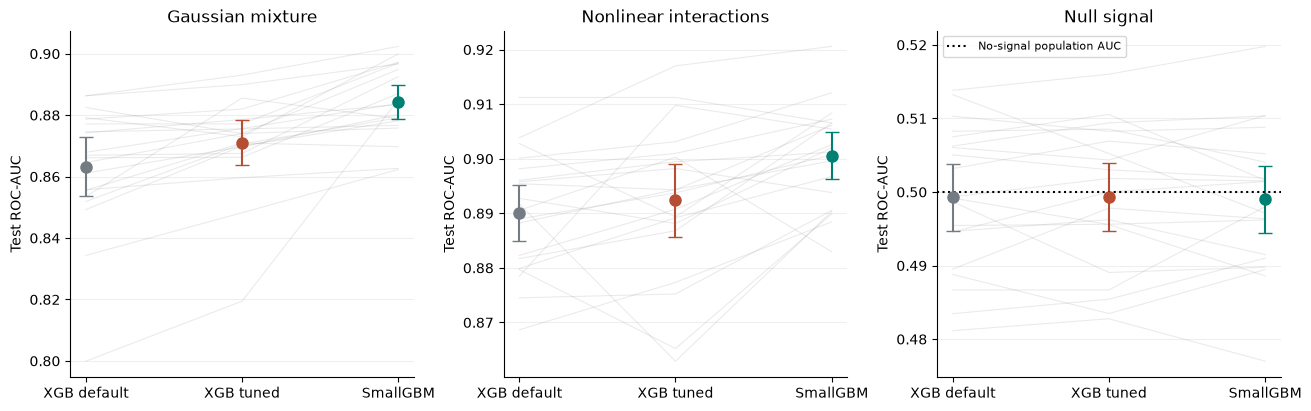
\includegraphics[width=0.98\textwidth]{tuning.png}
    \caption{Test ROC-AUC after training on 100 observations. Each grey line connects the three methods on the same trial. Points show means across 20 seeds and error bars show pointwise 95\% \(t\)-intervals.}
    \label{fig:tuning_comparison}
\end{figure}

On the Gaussian task, tuning improved mean test ROC-AUC from 0.863 to 0.871 (paired gain \(+0.0078\), 95\% CI \([+0.0031,+0.0124]\)). On the nonlinear task the corresponding scores were 0.890 and 0.892 (paired gain \(+0.0023\), 95\% CI \([-0.0033,+0.0080]\)). SmallGBM had the highest mean test ROC-AUC on these two tasks, at 0.884 and 0.901, respectively. On the null task all three means were approximately 0.499, close to the population ROC-AUC of 0.5 (Figure~\ref{fig:tuning_comparison}).

\begin{figure}[H]
    \centering
    \includegraphics[width=0.92\textwidth]{tuning_diagnostics.png}
    \caption{Paired ROC-AUC differences across 20 seeds. The left panel shows default minus tuned test ROC-AUC after fitting on all 100 observations. Negative values favor tuning. The right panel shows how much the validation gain exceeded the independent-test gain when both were measured using models trained on 80 observations. Dots show individual trials and black markers show means with pointwise 95\% \(t\)-intervals.}
    \label{fig:cv_optimism}
\end{figure}

To measure how well cross-validation estimated the benefit of tuning, we computed the selected configuration's mean validation ROC-AUC minus the default configuration's on the same folds. For comparison, we refitted both configurations on each original 80-observation training fold, scored them on the independent test set, and averaged their paired test differences over the five folds. Subtracting this matched-size test gain from the validation gain gives the quantity in the right panel of Figure~\ref{fig:cv_optimism}.

Cross-validation overstated the mean gain by 0.023 ROC-AUC on the Gaussian task, 0.017 on the nonlinear task, and 0.063 on the null task. On the null task, the apparent validation gain was 0.062 while the matched-size test gain was \(-0.0006\). Thus the search identified a validation advantage even when the features carried no information about the labels. On the Gaussian task, the apparent advantage was also optimistic, although tuning improved the final model's test score. The experiment measures selection optimism for one grid and one training size. Testing the scaling in Equation~\eqref{eq:val_bound} would require varying those quantities.

\subsubsection{Sample size and ROC-AUC on a Gaussian mixture}
\label{sec:n_crossover}

We drew equally likely binary labels and generated ten features from two Gaussian classes:
\[
Y\sim\operatorname{Bernoulli}(1/2),\qquad
X\mid Y=y\sim\mathcal{N}\bigl((2y-1)\mu,I_{10}\bigr),\qquad
\mu=v/\|v\|_2,\quad v=(1,0.75,-0.5,0,0,0,0,0,0,0)^\top .
\]
The Bayes score $S=\mu^\top X$ has distribution $\mathcal{N}(1,1)$ in class 1 and $\mathcal{N}(-1,1)$ in class 0. Thresholding at zero gives population accuracy $\Phi(1)=0.8413$. For independent draws from the two classes, their score difference has distribution $\mathcal{N}(2,2)$, so the population ROC-AUC is $\Phi(\sqrt{2})=0.9214$, where $\Phi$ is the standard normal distribution function.

For each of 20 seeds, all models received the same nested training samples of size $n\in\{100,200,500,1000,2000,5000,10000\}$ and the same independent test set of 10,000 observations. SmallGBM used its default configuration. Both XGBoost configurations used histogram trees of depth 3. \texttt{XGBoost-50} used 50 trees, a learning rate of 0.10, and half the features per tree. \texttt{XGBoost-200} used 200 trees, a learning rate of 0.05, and all features per tree.

\begin{figure}[H]
    \centering
    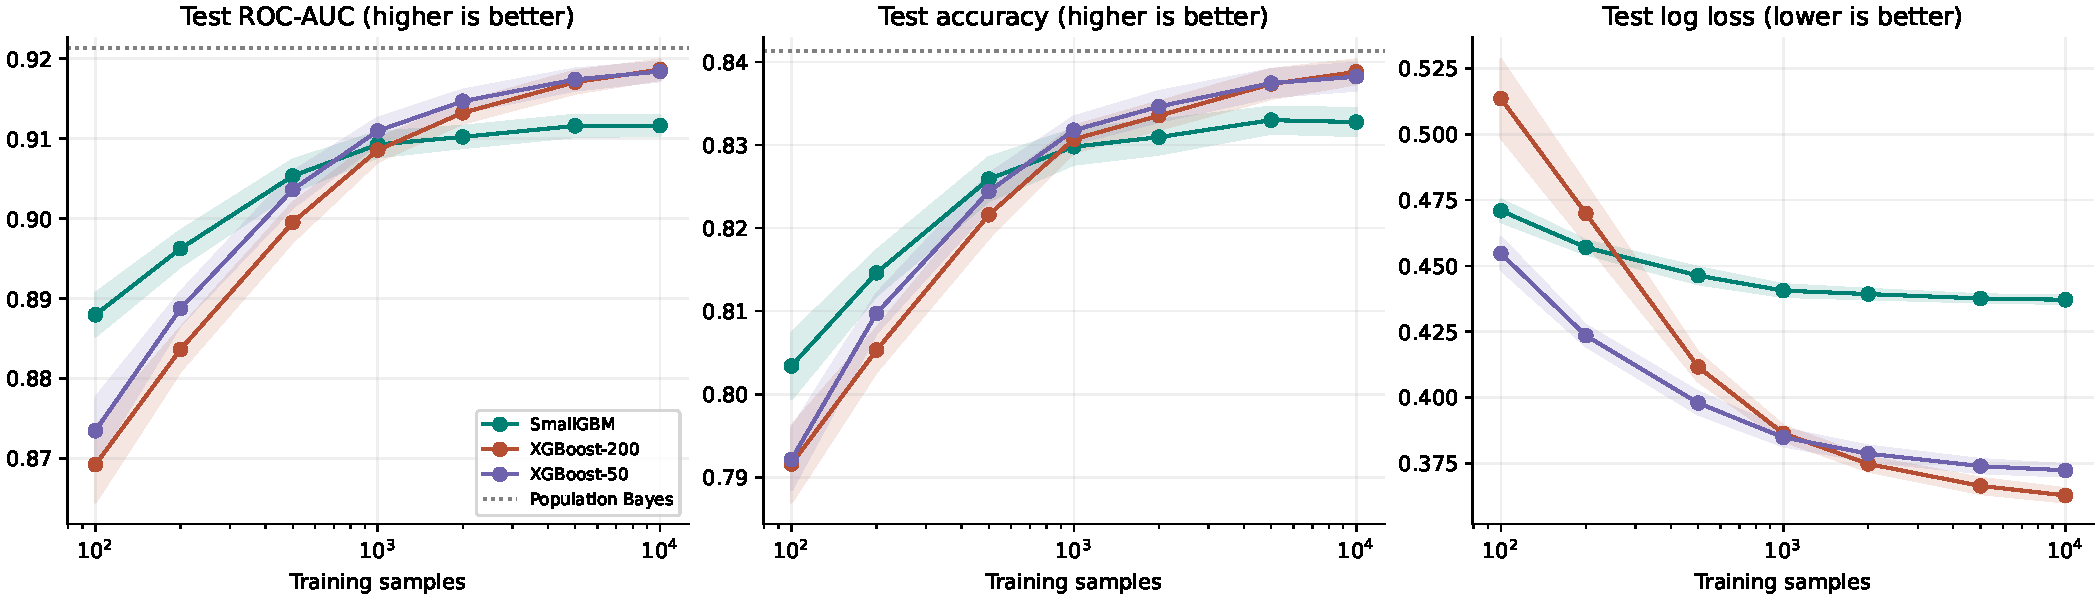
\includegraphics[width=0.98\textwidth]{n_crossover_scaling.pdf}
    \caption{Gaussian-mixture classification. Panels show test ROC-AUC (left), accuracy (center), and log loss (right). Markers are means over 20 seeds. Shading gives pointwise 95\% Student's $t$ confidence intervals for each mean. Dotted lines mark the population Bayes ROC-AUC (0.9214) and accuracy (0.8413). On the measured grid, both XGBoost configurations first exceed SmallGBM in mean accuracy at $n=1000$. For mean ROC-AUC this first occurs at $n=1000$ for \texttt{XGBoost-50} and $n=2000$ for \texttt{XGBoost-200}. \texttt{XGBoost-50} has lower mean log loss than SmallGBM at all seven sizes.}
    \label{fig:n_crossover}
\end{figure}

At $n=100$, SmallGBM had higher mean test ROC-AUC (0.8880) than \texttt{XGBoost-50} (0.8735) and \texttt{XGBoost-200} (0.8692). At $n=10{,}000$, the corresponding means were 0.9116, 0.9184, and 0.9186 (Figure~\ref{fig:n_crossover}).

We computed the XGBoost-minus-SmallGBM test ROC-AUC difference within each seed. For \texttt{XGBoost-50}, the mean difference changed from $-0.0017$ at $n=500$ to $+0.0017$ at $n=1000$. For \texttt{XGBoost-200}, it changed from $-0.0007$ at $n=1000$ to $+0.0030$ at $n=2000$. These pairs of measured sizes bracket the observed reversals in mean ROC-AUC for this distribution. The grid leaves the ordering at intermediate sizes unresolved.

\subsection{Surviving Data Pathologies}
\label{sec:pathologies}

\subsubsection{Heavy-Tailed Contamination and Label Corruption}
\label{sec:heavy_tailed_noise}

To empirically test the unbounded influence function bottleneck formalized in Section~\ref{sec:theory}, we evaluate model degradation under progressive target corruption across 10 unclipped random seeds ($0\%, 1\%, 5\%, 10\%,$ and $20\%$ contaminated training labels) while evaluating on clean hold-out test sets. To ensure strict mathematical reproducibility and isolate contamination effects from dataset-specific artifacts, we conduct two controlled stress tests with $d=10$ covariates ($n_{\text{train}} = 300$): (i) binary classification under stochastic label flips on a synthetic nonlinear interaction manifold defined by $X \sim \mathcal{N}(0, I_d)$ and $Y = \mathbb{I}(1.5 X_1 - X_2 + 0.8 X_3 X_4 + 0.5 \varepsilon > 0)$ with $\varepsilon \sim \mathcal{N}(0, 1)$, comparing tuning-free SmallGBM against default XGBoost (\texttt{binary:logistic}, $M=200$, $\text{depth}=3$, $\eta=0.05$); and (ii) continuous regression on the nonlinear Friedman \#1 benchmark ($\sigma_{\varepsilon} = 1.0$) under additive heavy-tailed Cauchy contamination $y_i^{\text{corr}} = y_i + \gamma \cdot \text{Cauchy}(0, 1)$ scaled by the clean training interquartile range $\gamma \propto \operatorname{IQR}(y_{\text{train}})$, comparing SmallMLP, default XGBoost (\texttt{reg:squarederror}), oracle-configured XGBoost (\texttt{reg:absoluteerror}), and a trivial median constant predictor.

\begin{figure}[H]
    \centering
    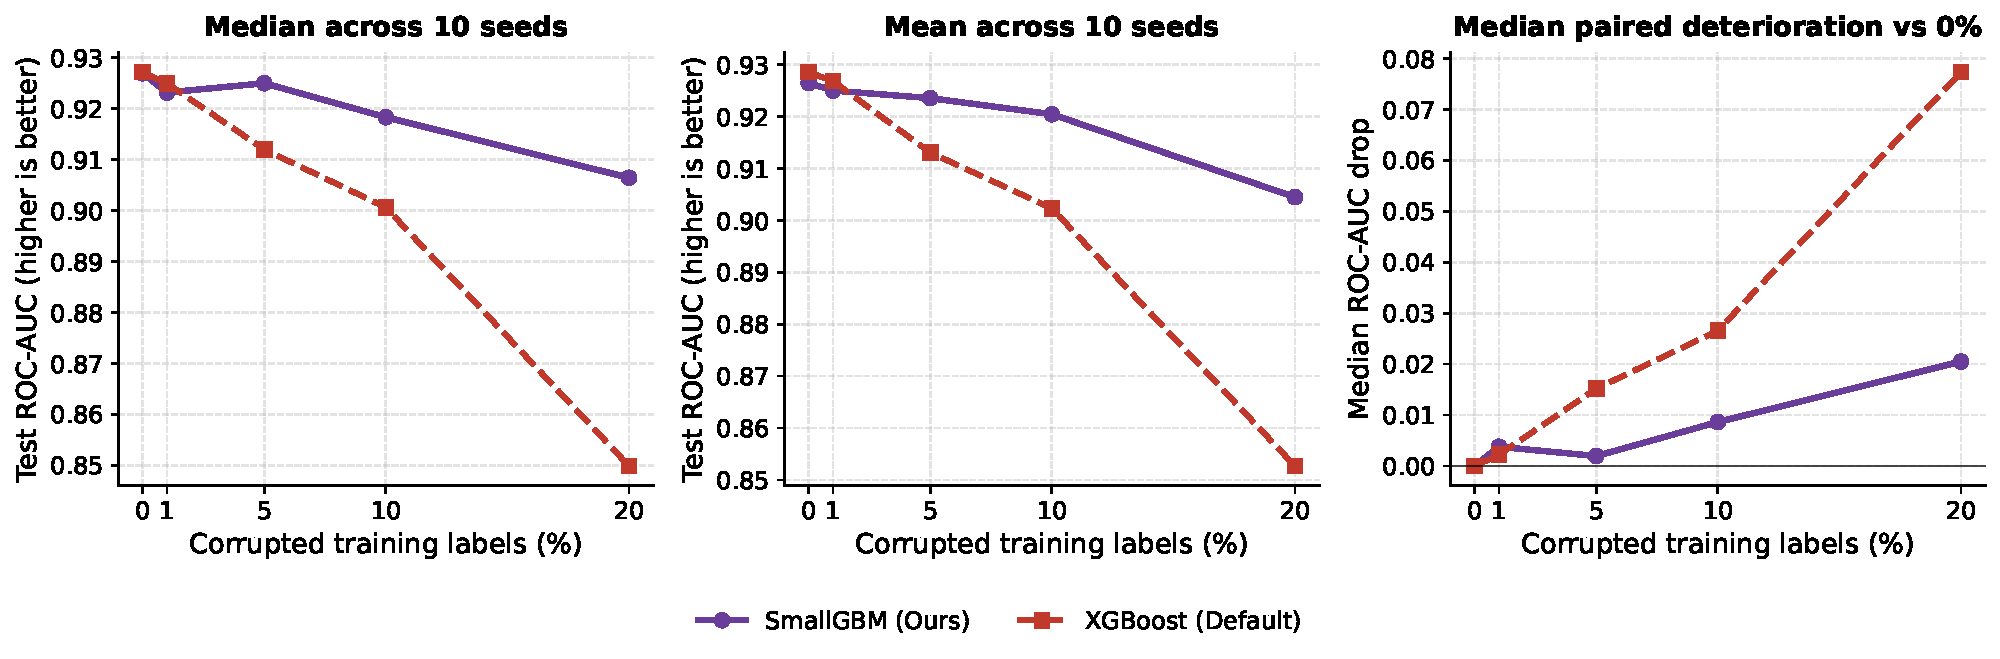
\includegraphics[width=0.98\textwidth]{label_noise_cls.pdf}
    \caption{\textbf{Binary Classification under Progressive Label Flips (10 Seeds).} On clean data ($0\%$), SmallGBM matches default XGBoost ($0.9265$ vs.\ $0.9286$ mean ROC-AUC). As label corruption increases to $20\%$, default XGBoost suffers a severe collapse to $0.8527$ (a median paired drop of $-0.0773$ AUC) as greedy splits isolate flipped labels. SmallGBM's median leaf estimator and MAD empirical Bayes shrinkage bound the influence of corrupted instances, maintaining $0.9045$ mean ROC-AUC ($3.7\times$ smaller median deterioration).}
    \label{fig:label_noise_cls}
\end{figure}

\textbf{Classification Resilience via Median Leaf Aggregation:} As shown in Figure~\ref{fig:label_noise_cls} and Table~\ref{tab:noise_sweep}, SmallGBM achieves statistical parity with default XGBoost on uncorrupted data ($0.9265$ vs.\ $0.9286$ mean ROC-AUC; $0.9270$ vs.\ $0.9272$ median), confirming that stochastic 5-threshold split selection and median leaf aggregation incur no baseline efficiency penalty. However, as label corruption rises, default XGBoost degrades rapidly: at $10\%$ corruption, its mean ROC-AUC drops to $0.9023$, and at $20\%$ it plunges to $0.8527$ (median $0.8499$, a paired deterioration of $-0.0773$ AUC). Because standard GBDTs perform exhaustive split searches and compute leaf weights via second-order Taylor sums (Equation~\ref{eq:taylor_leaf}), they actively isolate flipped labels into low-sample leaves with large log-odds updates. Conversely, SmallGBM restricts split candidates and computes small-leaf weights ($|I| \le 30$) via the sample median (Equation~\ref{eq:median_leaf}) coupled with MAD shrinkage toward the parent node (Equation~\ref{eq:mad_shrinkage}). Consequently, SmallGBM retains a mean ROC-AUC of $0.9204$ at $10\%$ corruption and $0.9045$ (median $0.9065$) at $20\%$ corruption—limiting median AUC loss to just $-0.0205$ ($3.7\times$ lower degradation than XGBoost) without any hyperparameter tuning.

\begin{figure}[H]
    \centering
    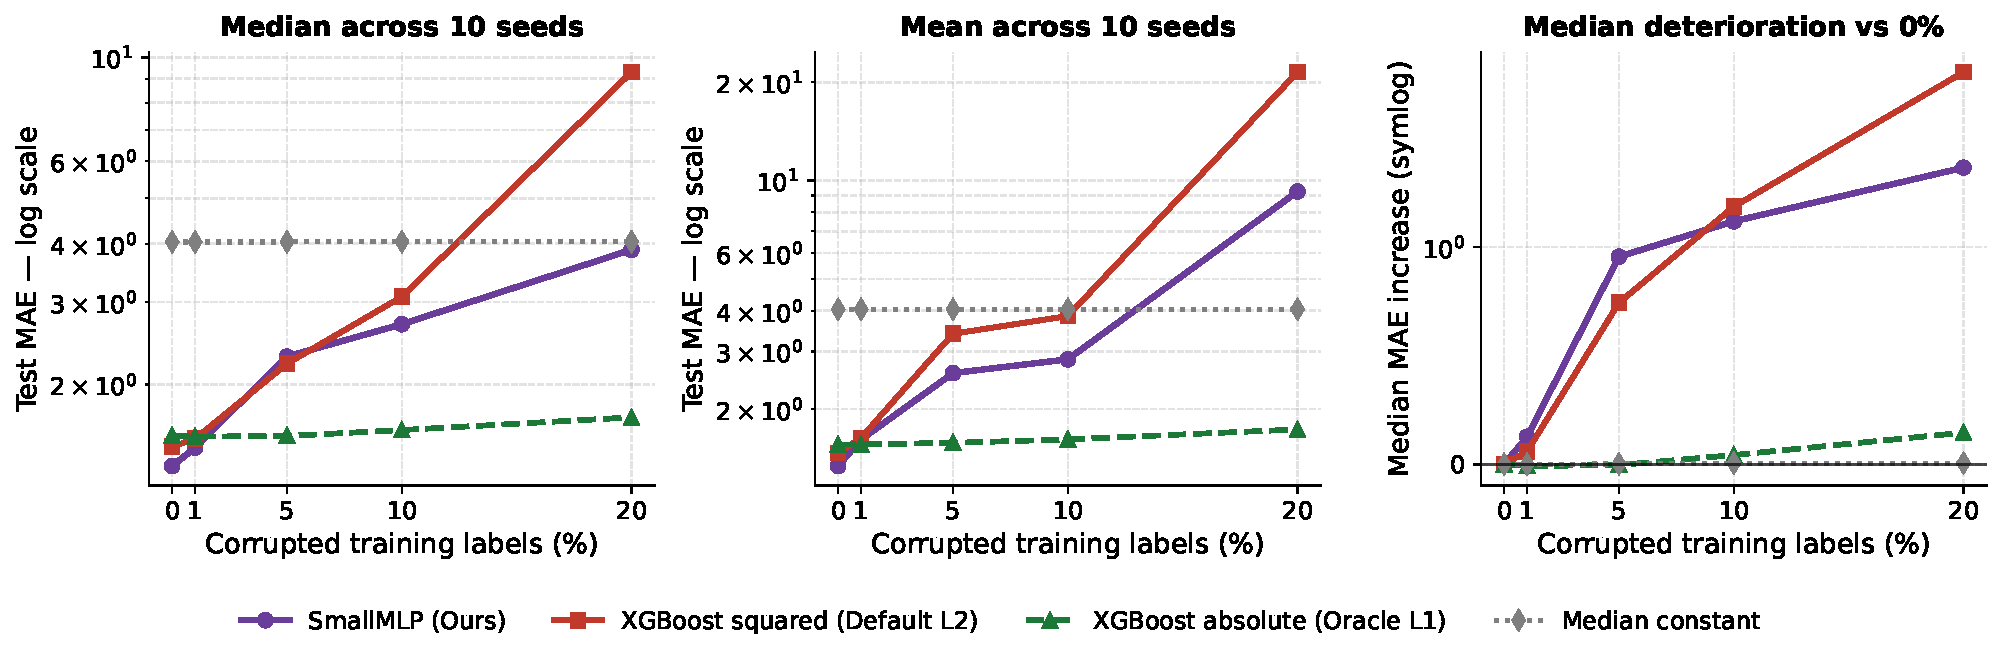
\includegraphics[width=0.98\textwidth]{cauchy_noise_reg.pdf}
    \caption{\textbf{Continuous Regression under Heavy-Tailed Cauchy Contamination (Friedman \#1, 10 Seeds).} At $0\%$ noise, SmallMLP achieves the lowest error ($\text{MAE} = 1.338$), outperforming both default XGBoost squared ($1.468$) and XGBoost absolute ($1.557$). Under Cauchy contamination, default XGBoost squared explodes by $14.6\times$ to $21.494$ mean MAE at $20\%$—performing $5.3\times$ worse than a trivial median constant ($4.039$). SmallMLP's capacity bottlenecks constrain mean outlier explosion ($9.260$ mean and $3.882$ median MAE at $20\%$), while illustrating the exact trade-off between smooth $L_2$ and bounded-gradient $L_1$ objectives.}
    \label{fig:cauchy_noise_reg}
\end{figure}

\begin{table}[H]
\centering
\caption{Mean and Median Test Performance Across Progressive Target Corruption (10/10 Seeds Retained)}
\vspace{4pt}
\resizebox{\textwidth}{!}{%
\begin{tabular}{llccccc}
\toprule
\textbf{Task / Metric} & \textbf{Model} & \textbf{0\% (Clean)} & \textbf{1\% Noise} & \textbf{5\% Noise} & \textbf{10\% Noise} & \textbf{20\% Noise} \\
\midrule
Classification (ROC-AUC $\uparrow$) & \textbf{SmallGBM (Ours)} & $0.9265$ ($0.9270$) & $0.9250$ ($0.9232$) & $\mathbf{0.9236}$ ($\mathbf{0.9250}$) & $\mathbf{0.9204}$ ($\mathbf{0.9183}$) & $\mathbf{0.9045}$ ($\mathbf{0.9065}$) \\
 & XGBoost (Default) & $\mathbf{0.9286}$ ($\mathbf{0.9272}$) & $\mathbf{0.9268}$ ($\mathbf{0.9250}$) & $0.9131$ ($0.9120$) & $0.9023$ ($0.9006$) & $0.8527$ ($0.8499$) \\
\midrule
Regression (Test MAE $\downarrow$) & \textbf{SmallMLP (Ours)} & $\mathbf{1.338}$ ($\mathbf{1.339}$) & $1.613$ ($\mathbf{1.466}$) & $2.576$ ($2.294$) & $2.839$ ($2.691$) & $9.260$ ($3.882$) \\
 & XGBoost (Default $L_2$) & $1.468$ ($1.473$) & $1.632$ ($1.532$) & $3.399$ ($2.216$) & $3.852$ ($3.080$) & $21.494$ ($9.301$) \\
 & XGBoost (Oracle $L_1$) & $1.557$ ($1.556$) & $\mathbf{1.559}$ ($1.548$) & $\mathbf{1.576}$ ($\mathbf{1.553}$) & $\mathbf{1.614}$ ($\mathbf{1.599}$) & $\mathbf{1.732}$ ($\mathbf{1.702}$) \\
 & Median Constant & $4.036$ ($4.033$) & $4.036$ ($4.033$) & $4.038$ ($4.035$) & $4.039$ ($4.038$) & $4.039$ ($4.038$) \\
\bottomrule
\multicolumn{7}{l}{\footnotesize \textit{Note:} Values report $\text{Mean} \; (\text{Median})$ across 10 unclipped random seeds.}
\end{tabular}%
}
\label{tab:noise_sweep}
\end{table}

\textbf{Regression under Cauchy Contamination and the Loss-Selection Dilemma:} Figure~\ref{fig:cauchy_noise_reg} and Table~\ref{tab:noise_sweep} expose the fragility of unregularized second-order Taylor approximations under heavy-tailed continuous noise. On clean data ($0\%$), SmallMLP achieves the lowest error ($\text{MAE} = 1.338$), outperforming default $L_2$ XGBoost ($1.468$). When Cauchy noise is injected, default $L_2$ XGBoost suffers unbounded gradient explosions ($g_i = \hat{y}_i - y_i$ with constant Hessian $h_i = 1$): while its median MAE at $5\%$ corruption ($2.216$) briefly remains comparable to SmallMLP ($2.294$), extreme outlier seeds already drive its mean MAE up to $3.399$ (versus $2.576$ for SmallMLP). By $20\%$ corruption, default $L_2$ XGBoost explodes to a mean MAE of $21.494$ (median $9.301$)—performing more than $5\times$ worse than a trivial median constant predictor ($4.039$).

While SmallMLP also optimizes a standard $L_2$ objective, its strict capacity bottlenecks ($w_1 = \min(2n, 128)$, inverse weight decay $\lambda = 1/n$, and clamped dropout) prevent individual neurons from dedicating capacity to isolated Cauchy spikes, cutting mean error by more than half relative to default XGBoost at $20\%$ corruption ($9.260$ vs.\ $21.494$) and maintaining a median MAE ($3.882$) below the constant baseline. Crucially, SmallMLP deliberately retains a smooth $L_2$ objective rather than switching to $L_1$ or Huber loss: while non-smooth $L_1$ gradients bound extreme $20\%$ Cauchy spikes—as demonstrated by Oracle $L_1$ XGBoost (\texttt{reg:absoluteerror}) achieving $1.732$ MAE at $20\%$—constant-magnitude subgradients degrade optimization efficiency on clean smooth manifolds and distort the penultimate embedding geometry $h(x)$ required for locally weighted conformal prediction (Equation~\ref{eq:h_cal}). Indeed, Table~\ref{tab:noise_sweep} confirms that Oracle $L_1$ XGBoost suffers significantly higher baseline error on uncorrupted data ($1.557$ vs.\ SmallMLP's $1.338$). Thus, in a strict zero-tuning regime where target tail behavior is unknown \textit{a priori}, SmallMLP's architectural bottlenecking provides a balanced middle ground: preserving state-of-the-art accuracy on clean data while bounding mean divergence under moderate contamination ($\le 10\%$).

\subsubsection{Prediction Interval Coverage Under Heteroscedasticity and $d \approx n$}
\label{sec:conformal_uq}

We evaluate the test coverage and width of the prediction intervals described in Section~\ref{sec:uq} on a heteroscedastic nonlinear regression problem ($n = 150$, $n_{\text{test}} = 2000$, 20 independent random seeds, target coverage $1 - \alpha = 0.90$). Covariates are drawn as $X \sim \mathcal{N}(0, I_d)$ across both a low-dimensional regime ($d = 10$) and a high-dimensional regime ($d = 100$, where $d \approx n$), with targets generated via $Y = 1.5 X_1 - X_2 + 0.8 X_3 X_4 + \sin(X_5) + \sigma(X)\varepsilon$, $\varepsilon \sim \mathcal{N}(0, 1)$, where $\sigma(X) = 0.25$ for $X_1 \le 0$ and $\sigma(X) = 1.50$ for $X_1 > 0$ (a $6\times$ noise-scale shift). We compare a parametric Gaussian Process (\texttt{GP (Type-II ML)}, ARD-RBF + WhiteKernel fitted on all $n = 150$ samples) against \texttt{SmallMLP} calibrated via a single non-tuned $75/25$ split ($n_{\text{fit}} = 112$, $n_{\text{cal}} = 38$) under both unweighted split conformal prediction (Equation~\eqref{eq:conformal_cov}) and locally weighted conformal prediction over the penultimate bottleneck embedding $h(x)$ (Equation~\eqref{eq:h_cal}).

\begin{figure}[H]
    \centering
    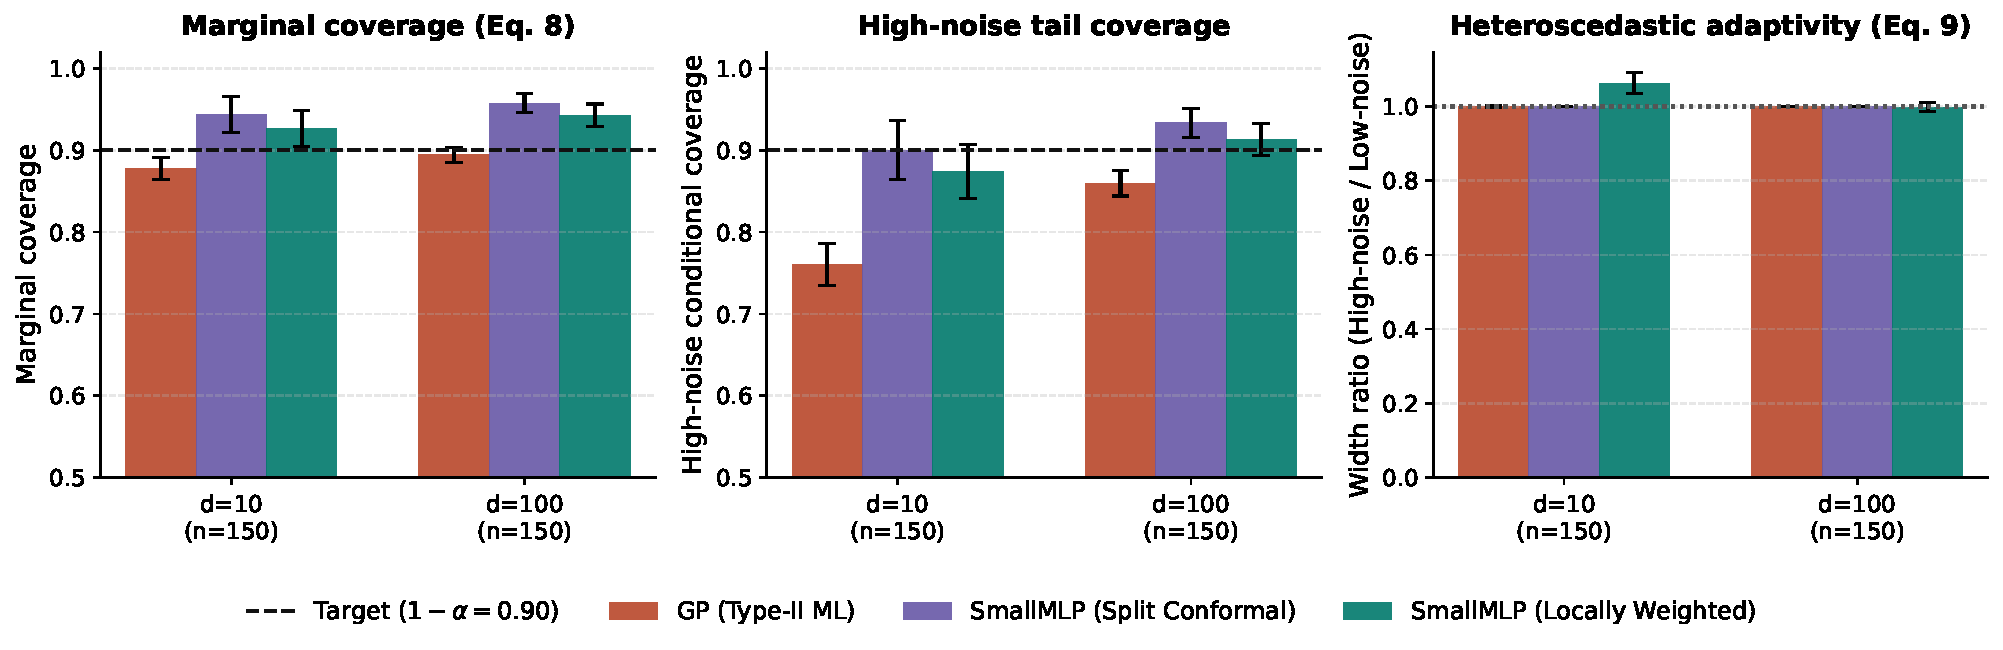
\includegraphics[width=0.98\textwidth]{conformal_uq.pdf}
    \caption{Prediction intervals under a sixfold difference in noise scale at $d=10$ and $d=100$ ($n=150$). The panels show observed coverage on the full test set (left), coverage among high-noise observations with $X_1>0$ (center), and the ratio of mean widths in the high- and low-noise groups (right). Results are means over 20 seeds with 95\% confidence intervals. The reference coverage is $90\%$. At $d=10$, the locally weighted SmallMLP interval covered $92.7\%$ overall and $87.4\%$ in the high-noise group.}
    \label{fig:conformal_uq}
\end{figure}

For the standard unweighted rule at $m=38$ and target $1-\alpha=0.90$, $k=\lceil39\times0.90\rceil=36$. With exchangeable, almost surely distinct residuals, the 36th calibration residual therefore gives marginal coverage $36/39\approx92.3\%$ (Equation~\eqref{eq:conformal_cov}). The denominator includes the new observation. The fraction $36/38$ is the cumulative fraction of calibration residuals at that cutoff. A finite benchmark can give an empirical coverage different from $36/39$.

Figure~\ref{fig:conformal_uq} reports three comparisons.
\begin{itemize}
    \item \textbf{Marginal coverage and width.} At $d=10$, unweighted SmallMLP intervals covered $94.3\%$ of test responses with mean width $6.28$. Local weighting reduced mean width to $5.58$ and coverage to $92.7\%$. At $d=100$, the corresponding change was from $9.32$ to $8.54$ in width and from $95.7\%$ to $94.3\%$ in coverage. The Gaussian process had mean marginal coverage of $87.8\%$ and $89.5\%$ at $d=10$ and $d=100$, respectively.
    \item \textbf{Coverage in the high-noise group.} Among test points with $X_1>0$, coverage of the locally weighted intervals was $87.4\%$ at $d=10$ and $91.3\%$ at $d=100$. The corresponding Gaussian process coverages were $76.0\%$ and $86.0\%$. At $d=10$ the weighted method exceeded the target overall while falling below it in the high-noise group.
    \item \textbf{Variation in width.} At $d=10$, the locally weighted intervals had mean width $5.74$ in the high-noise group and $5.41$ in the low-noise group (ratio $1.06$). The correlation between width and noise scale was $0.210$. At $d=100$, the ratio rounded to $1.00$ and the correlation was approximately zero. The unweighted interval has constant width within each fitted split by construction.
\end{itemize}

\subsection{Component Ablations and Meta-Validation}

\subsubsection{The $\alpha$ and $\beta$ Capacity Surface on the Meta-Training Set}
As established in Section 2.2, continuous regression ($K=1$) utilizes the deterministic $w_1 = \min(2n, 128)$ width bound, whereas the capacity scaling constants $\alpha$ and $\beta$ in Equations~\eqref{eq:width_w1} and~\eqref{eq:width_wl} specifically govern multiclass representation capacity ($K \ge 2$). To verify that this scaling rule does not rely on fragile hyperparameter tuning or test-set leakage, we evaluate the joint sensitivity of $\alpha \in [2.0, 10.0]$ and $\beta \in [0.5, 0.9]$ across the classification tasks of the disjoint Meta-Training Set.

\begin{figure}[H]
\centering
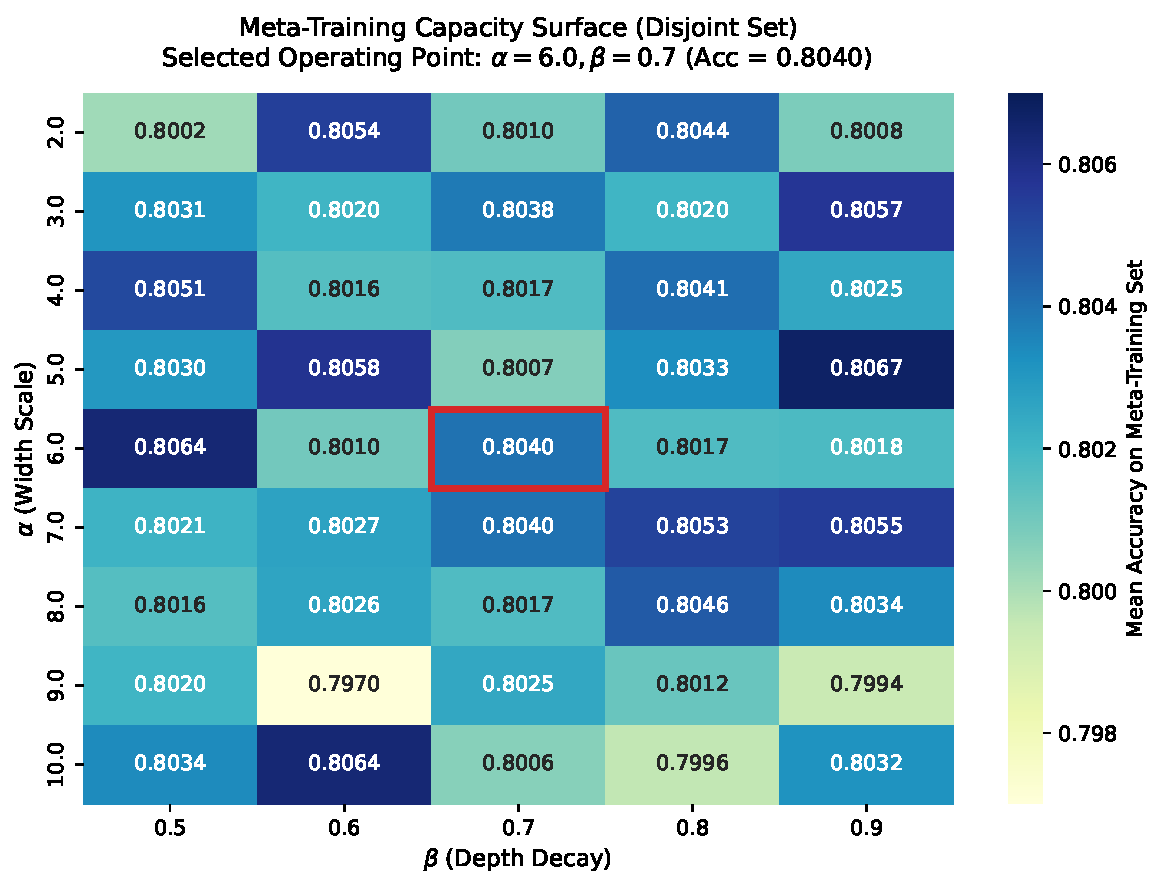
\includegraphics[width=0.68\textwidth]{meta_grid_surface.pdf}
\caption{Empirical capacity surface across the disjoint Meta-Training Set plotted on a standardized accuracy scale ($[0.76, 0.84]$). Total mean accuracy fluctuates by less than $0.97\%$ across the entire 45-point grid ($[0.7970, 0.8067]$), visually confirming a flat stability plateau. The red bounding box denotes the selected structural prior ($\alpha=6.0, \beta=0.7$).}
\label{fig:meta_surface}
\end{figure}

As illustrated in Figure~\ref{fig:meta_surface}, when viewed on a non-distorted accuracy scale, the performance surface forms a remarkably uniform stability plateau: across a five-fold increase in $\alpha$ and the full spectrum of $\beta$, mean meta-training accuracy varies within a narrow band of $0.97\%$ (from $0.7970$ to $0.8067$). The minor cell-to-cell fluctuations ($\pm 0.2\%$) reflect stochastic weight initialization variance inherent to $n < 500$ rather than structural sensitivity. This confirms that the asymptotic scaling factor $\sqrt{n K \sqrt{d}}$ captures the intrinsic geometry of the low-sample regime, rendering the network largely invariant to local constant perturbations.

To lock in a single operating point prior to hold-out evaluation, we apply two structural boundary conditions. First, we reject boundary configurations with minimal decay ($\beta = 0.9$, such as $(\alpha=5.0, \beta=0.9)$ at $0.8067$), as they fail to compress the second hidden layer and inflate parameter count. Second, while aggressive compression ($\beta \le 0.6$, such as $(\alpha=6.0, \beta=0.5)$ at $0.8064$) yields marginally higher point averages on specific random seeds, slashing penultimate layer width by $\ge 40\%$ risks representation collapse and metric distortion in the embedding space $h(x)$ required for locally weighted conformal calibration (Equation~\eqref{eq:h_cal}). Consequently, we freeze the central operating point $\alpha=6.0, \beta=0.7$ ($0.8040$ accuracy, within $0.27\%$ noise tolerance of the grid maximum) as a conservative structural prior that balances parameter compression ($30\%$ decay) with metric preservation for uncertainty quantification.

\subsubsection{Depth Ablation: Architectural Saturation Beyond Two Hidden Layers}
\label{sec:depth_ablation}

While Equations~\eqref{eq:width_w1} and~\eqref{eq:width_wl} govern layer width deterministically, eliminating Neural Architecture Search also requires fixing network depth $L$ prior to deployment. Starting from the minimal two-layer bottleneck architecture ($L=2$) required to support geometric layer compression ($\beta$) and extract a low-dimensional penultimate embedding $h(x)$ for locally weighted conformal calibration (Equation~\ref{eq:h_cal}), we sweep the number of hidden layers $L \in \{2, 3, 4, 5\}$ across sample sizes $n \in \{100, 200, 400\}$ ($d=10$, $n_{\text{test}} = 5000$, 10 independent random seeds). We evaluate both Friedman \#1 regression (Test MAE) and nonlinear classification (Test Accuracy), keeping all capacity scaling, regularization rules, and internal optimization settings ($\text{max epochs} = 500$, $\text{patience} = 30$, with zero hyperparameter search) fixed across depths.

\begin{figure}[H]
    \centering
    \includegraphics[width=0.96\textwidth]{depth_ablation.pdf}
    \caption{\textbf{Depth Ablation ($L \in \{2, 3, 4, 5\}$) Across Sample Sizes $n \in \{100, 200, 400\}$ (10 Seeds, Mean $\pm$ Pointwise 95\% $t$-Intervals).} Left: Mean test MAE on Friedman \#1 regression. Right: Mean test accuracy on nonlinear classification. Extending depth beyond two hidden layers provides no consistent generalization benefit: regression error increases monotonically with depth at $n=200$ and $n=400$, while classification at $n=100$ suffers severe optimization instability and accuracy collapse for $L \ge 4$.}
    \label{fig:depth_ablation}
\end{figure}

As shown in Figure~\ref{fig:depth_ablation}, increasing network depth beyond $L=2$ hidden layers fails to improve generalization while substantially inflating parameter count:
\begin{itemize}
    \item \textbf{Friedman \#1 Regression:} At $n=100$, test MAE remains statistically flat across depths ($2.166$ at $L=2$ vs.\ $2.126$ at $L=3$ and $2.153$ at $L=5$, all within overlapping 95\% $t$-intervals). However, as the training signal strengthens at $n=200$ and $n=400$, deeper architectures degrade monotonically: mean MAE rises from $1.571$ ($L=2$) to $1.716$ ($L=5$) at $n=200$, and from $1.231$ ($L=2$) to $1.325$ ($L=5$) at $n=400$. Meanwhile, trainable parameter count expands by $3.8\times$ (from $\approx 18\text{k}$ at $L=2$ to $\approx 67.5\text{k}$ at $L=5$), confirming that excess depth introduces unnecessary variance without reducing approximation bias.
    \item \textbf{Nonlinear Classification:} At $n=200$ and $n=400$, accuracy exhibits a flat-to-slightly-declining profile as depth increases ($0.861 \to 0.858$ at $n=200$; $0.880 \to 0.875$ at $n=400$), even as parameter count grows nearly $1.8\times$ (reaching $\approx 120\text{k}$ parameters at $n=400, L=5$). Crucially, in the extreme low-sample regime ($n=100$), deeper networks suffer severe optimization collapse: mean accuracy drops by nearly $7$ percentage points from $0.816$ ($L=2$) to $0.750$ ($L=4$) and $0.747$ ($L=5$), accompanied by a dramatic explosion in seed-to-seed variance.
\end{itemize}
Collectively, these results confirm that depth is not a productive degree of freedom for $n < 500$. Fixing SmallMLP at $L=2$ hidden layers achieves the best balance of accuracy, optimization stability, and parameter parsimony without requiring validation-based architecture search.

\subsection{True Negative Results and Structural Limitations}
\label{sec:negative_results}

We examine the efficiency of estimating a Gaussian location and relate this separate experiment to the observed classification results in Figure~\ref{fig:n_crossover}.

\subsubsection{Gaussian Location Estimation and Classifier Performance}
\label{sec:gaussian_penalty}

We drew independent samples from $\mathcal{N}(0,1)$ and used the sample mean and the sample median to estimate the common center at zero. At each sample size we averaged squared estimation errors over 5,000 draws.

\begin{figure}[H]
    \centering
    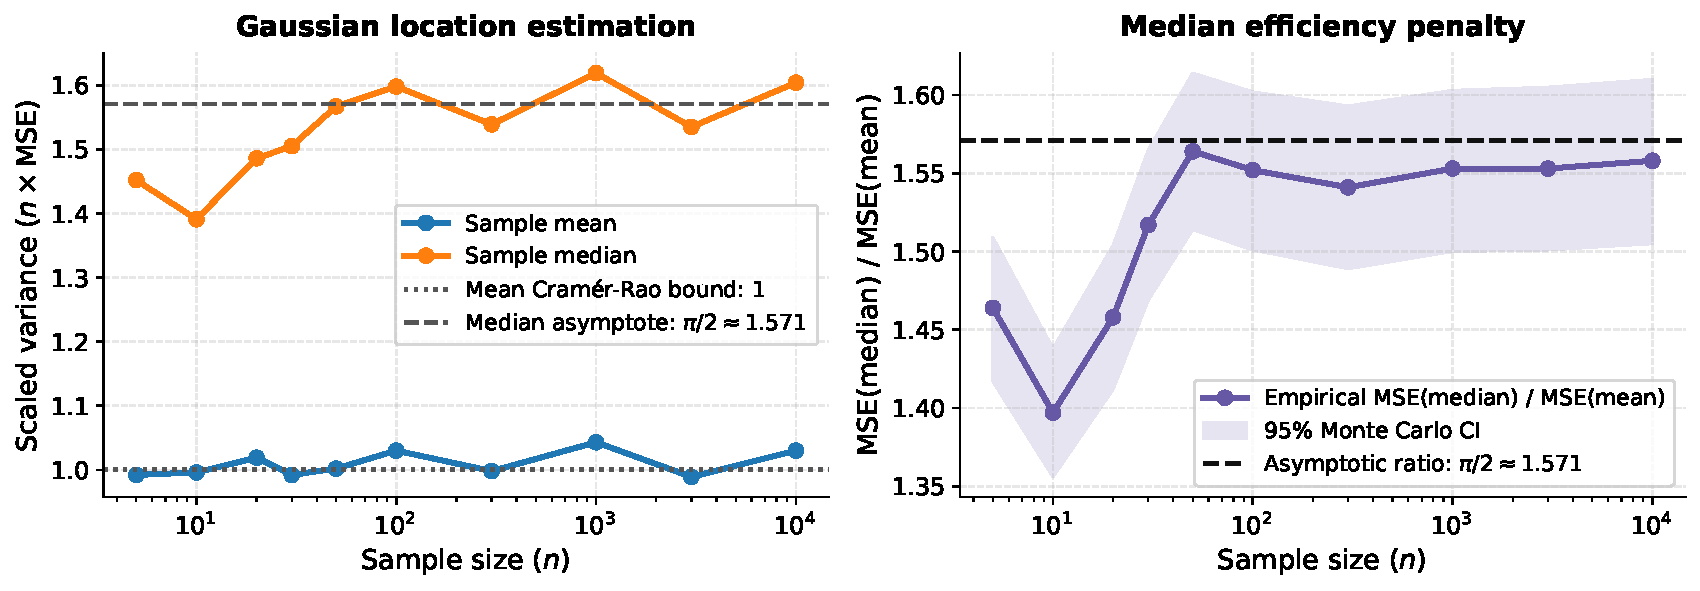
\includegraphics[width=0.96\textwidth]{gaussian_efficiency_penalty.pdf}
    \caption{\textbf{The Gaussian Efficiency Penalty of Robust Estimation.} Left: On uncorrupted Gaussian data, the sample mean achieves the Cram\'{e}r-Rao lower bound ($n \times \text{MSE} \to 1$), whereas the sample median converges to the asymptotic variance limit $\pi/2 \approx 1.571$. Right: The empirical MSE ratio $\text{MSE}(\text{median}) / \text{MSE}(\text{mean})$ across sample sizes, reaching $1.558$ ($95\%$ Monte Carlo CI: $[1.505, 1.610]$) at $n = 10^4$. Both panels concern estimation of a Gaussian location.}
    \label{fig:gaussian_penalty}
\end{figure}

As shown in Figure~\ref{fig:gaussian_penalty}, while the sample mean is the minimum-variance unbiased estimator under Gaussian noise ($n \times \text{MSE} \approx 1.00$ across all $n$), the sample median incurs a strict variance penalty governed by the asymptotic distribution of sample quantiles:
\begin{equation}
\label{eq:asymptotic_efficiency}
\lim_{n\to\infty} \frac{\operatorname{Var}\left(\operatorname{median}(X_1,\ldots,X_n)\right)}{\operatorname{Var}(\bar X_n)} = \frac{1}{4 f(0)^2 \sigma^2} = \frac{\pi}{2} \approx 1.5708
\end{equation}
where $f(0)$ is the density of $\mathcal{N}(0,\sigma^2)$ at its median. The resulting asymptotic relative efficiency of the median is $2/\pi$. This calculation describes an independent Gaussian sample. At each boosting step the classification pseudo-residuals depend on binary labels and the current fitted probabilities. Attributing the ROC-AUC reversals in Figure~\ref{fig:n_crossover} to the leaf estimator would require varying that component while holding the other tree settings fixed.

The choice of metric also affects the comparison. At $n=100$, \texttt{XGBoost-50} had lower mean test log loss than SmallGBM (0.455 versus 0.471), even though SmallGBM ranked the classes better by ROC-AUC. At $n=10{,}000$, the corresponding log losses were 0.372 and 0.437. Log loss measures the quality of probability predictions. Identifying systematic underconfidence would require a separate calibration analysis.

\section{Conclusion}
\label{sec:conclusion}

Machine learning on small tabular datasets ($n < 1000$) is governed by structural bottlenecks that standard big-data workflows cannot resolve through hyperparameter tuning. In this paper, we formalized these constraints as the Trilemma of Small Data Learning—the inability to simultaneously achieve low variance, low bias, and calibrated uncertainty without depleting scarce training signals via validation splits—and evaluated two zero-tuning algorithmic baselines, SmallGBM and SmallMLP, as targeted case studies.

Our empirical benchmarks measure how model performance changes with sample size, dimensionality, and label contamination. At $n=100$, five-fold cross-validation overstated the gain from tuning XGBoost by 0.063 ROC-AUC on random labels. On the Gaussian mixture, tuning improved test ROC-AUC from 0.863 to 0.871 after refitting. SmallGBM achieved 0.884 on the same trials. On the Gaussian mixture, the paired mean ROC-AUC difference favored \texttt{XGBoost-50} over SmallGBM by $n=1000$ and \texttt{XGBoost-200} by $n=2000$. At the preceding measured size for each comparison ($500$ and $1000$, respectively), SmallGBM had the higher mean ROC-AUC. In the separate label-flip experiment, the median ROC-AUC decrease at $20\%$ corruption was $3.7$ times as large for the tested XGBoost configuration as for SmallGBM. For neural architectures, our meta-validation and depth ablations confirm that deterministic capacity scaling ($\alpha = 6.0, \beta = 0.7$) and a fixed two-layer bottleneck ($L = 2$) eliminate neural architecture search while preventing the optimization collapse observed in deeper networks at $n = 100$. Under a sixfold difference in noise scale, locally weighted SmallMLP intervals were narrower on average than unweighted intervals. Their observed marginal coverage was $92.7\%$ at $d=10$ and $94.3\%$ at $d=100$. At $d=10$, coverage fell to $87.4\%$ in the high-noise group. The finite-sample guarantee in Equation~\eqref{eq:conformal_cov} applies to the unweighted procedure under exchangeability.

At the largest measured training size ($n=10{,}000$), all three classifiers remained below the population Bayes ROC-AUC for the Gaussian mixture. The separate location experiment quantified the variance cost of estimating the center of a normal sample with the median. Similarly, SmallMLP's smooth $L_2$ objective remains vulnerable to extreme ($20\%$) heavy-tailed Cauchy outliers compared to $L_1$-loss boosting. By delineating both the strengths and mathematical limits of zero-tuning inductive biases, this work provides a rigorous, empirically grounded foundation for future research in low-sample tabular learning.

\section*{Acknowledgements}

The authors thank Beijing Institute of Technology for providing
a supportive academic environment and opportunities for research
and collaboration.

\section*{Author Contributions}

\textbf{Ilya Emelyanov} conceived the study, developed the mathematical
framework, and implemented the SmallGBM and SmallMLP libraries.
\textbf{Dmitrii Dobrydin} designed and conducted the benchmarks
and experiments.
\textbf{Muhammad Hamza} contributed to validation, helped revise
the manuscript structure, and provided methodological feedback.

\bibliographystyle{unsrt}
\bibliography{references,coverage_sources}
\end{document}